% REP001 探索：ルールベース3手法の動作と評価（親：W001。問いは未確定）
% コンパイル：uplatex を2回 → dvipdfmx（TEXINPUTS で .claude/templates/progress_report// を参照）
\documentclass[twocolumn, 10pt]{ujarticle}
\usepackage{progress_report}

\begin{document}

\reportid{REP001}
\questionid{W001}
\exploration{既存のルールベース入札手法は，この環境でどう動くか}
\reportdate{20261007}
\summary{%
最終的には新しい入札方法を提案したいが，その前に，既存のルールベース手法（PID，ABid，Online LP）をこのシミュレータで動かすと何が起きるかを確認した。
広告主48社の位置×4エピソードで3手法を比べ，6位置で主要パラメータを振ったところ，全270回が完走し，Online LPのスコア合計がPIDの1.92倍，ABidの1.49倍で最大であった（「Online LPが最良」は論文と一致。PIDとABidの順序は論文と異なる）。
1回の評価は約150〜215秒・約2.5GBで，結果は再現した。
}
\beginverification

% ============================================================
\section{目的}\label{sec:e-purpose}
% ============================================================

既存のルールベース入札手法（PID，ABid，Online LP）が，このシミュレータでどう動くかを知る。

% ============================================================
\section{実験}\label{sec:e-exp}
% ============================================================

\subsection{対象のアルゴリズム}\label{sec:e-algo}

3手法とも，各ティックの頭に，広告機会（PV）ごとの入札額を「$\alpha\times$価値」で決める（価値は購入確率）。
違いは，入札係数$\alpha$の決め方である（表\ref{tab:algo}）。

\begin{table}[H]
\centering
\caption{3手法の$\alpha$の決め方（数値は既定値）}
\label{tab:algo}
\footnotesize
\begin{tabularx}{\linewidth}{@{}l>{\raggedright\arraybackslash}p{0.2\linewidth}>{\raggedright\arraybackslash}X@{}}
\toprule
手法 & 見るもの & $\alpha$の決め方 \\
\midrule
PID & 残り予算，前のティックの支払い & 最初は15。今のペースで使い切る量が残り予算の0.7倍未満なら1.2倍，1.1倍超なら0.7倍 \\
\addlinespace
ABid & CPA制約，今のティックの価値 & CPA制約$\times$（価値$\div$価値の平均）。価値が高いPVほど強気。予算は見ない \\
\addlinespace
Online LP & 残り予算，早見表，CPA制約 & 過去の1日の記録で，割安なPVから順に買ったとき，残り予算で買える境目の値段。上限はCPA制約の1.5倍 \\
\bottomrule
\end{tabularx}
\end{table}

% 2段抜きの図は，2ページ目の上に出すためにここで宣言する
\begin{figure*}[t]
\centering
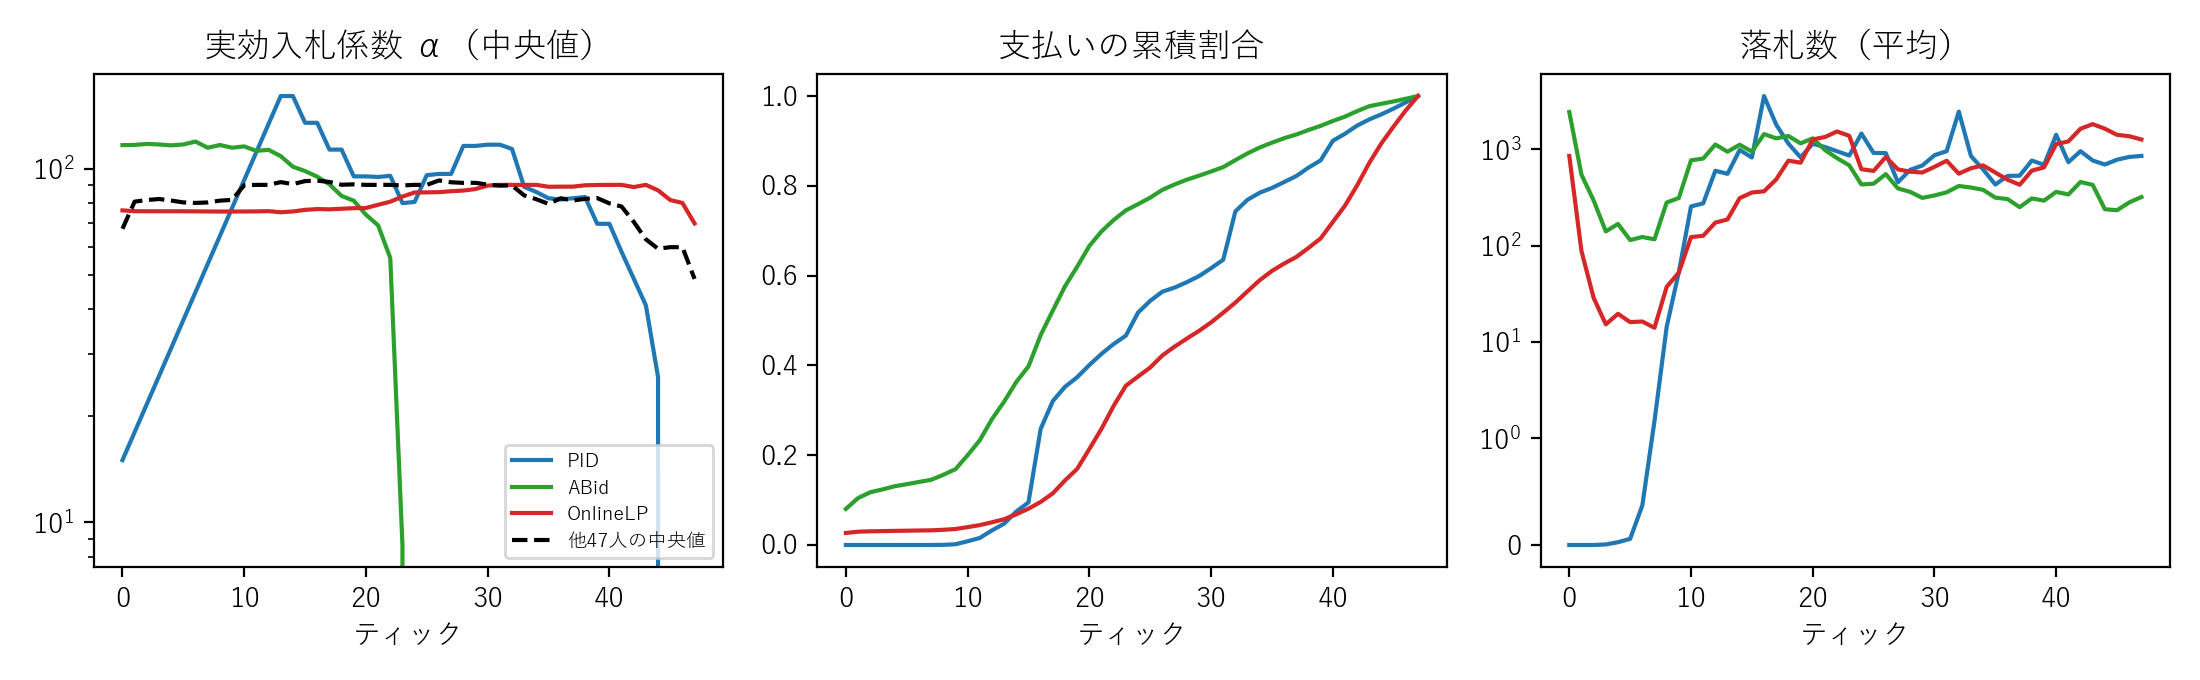
\includegraphics[width=0.8\textwidth]{fig/fig_alpha_time.png}
\caption{既定設定の3手法の時系列（192セルの中央値または平均）。左：実効入札係数$\alpha$（対数軸），中：支払いの累積割合，右：落札数}
\label{fig:alpha}
\end{figure*}
\begin{figure*}[t]
\centering
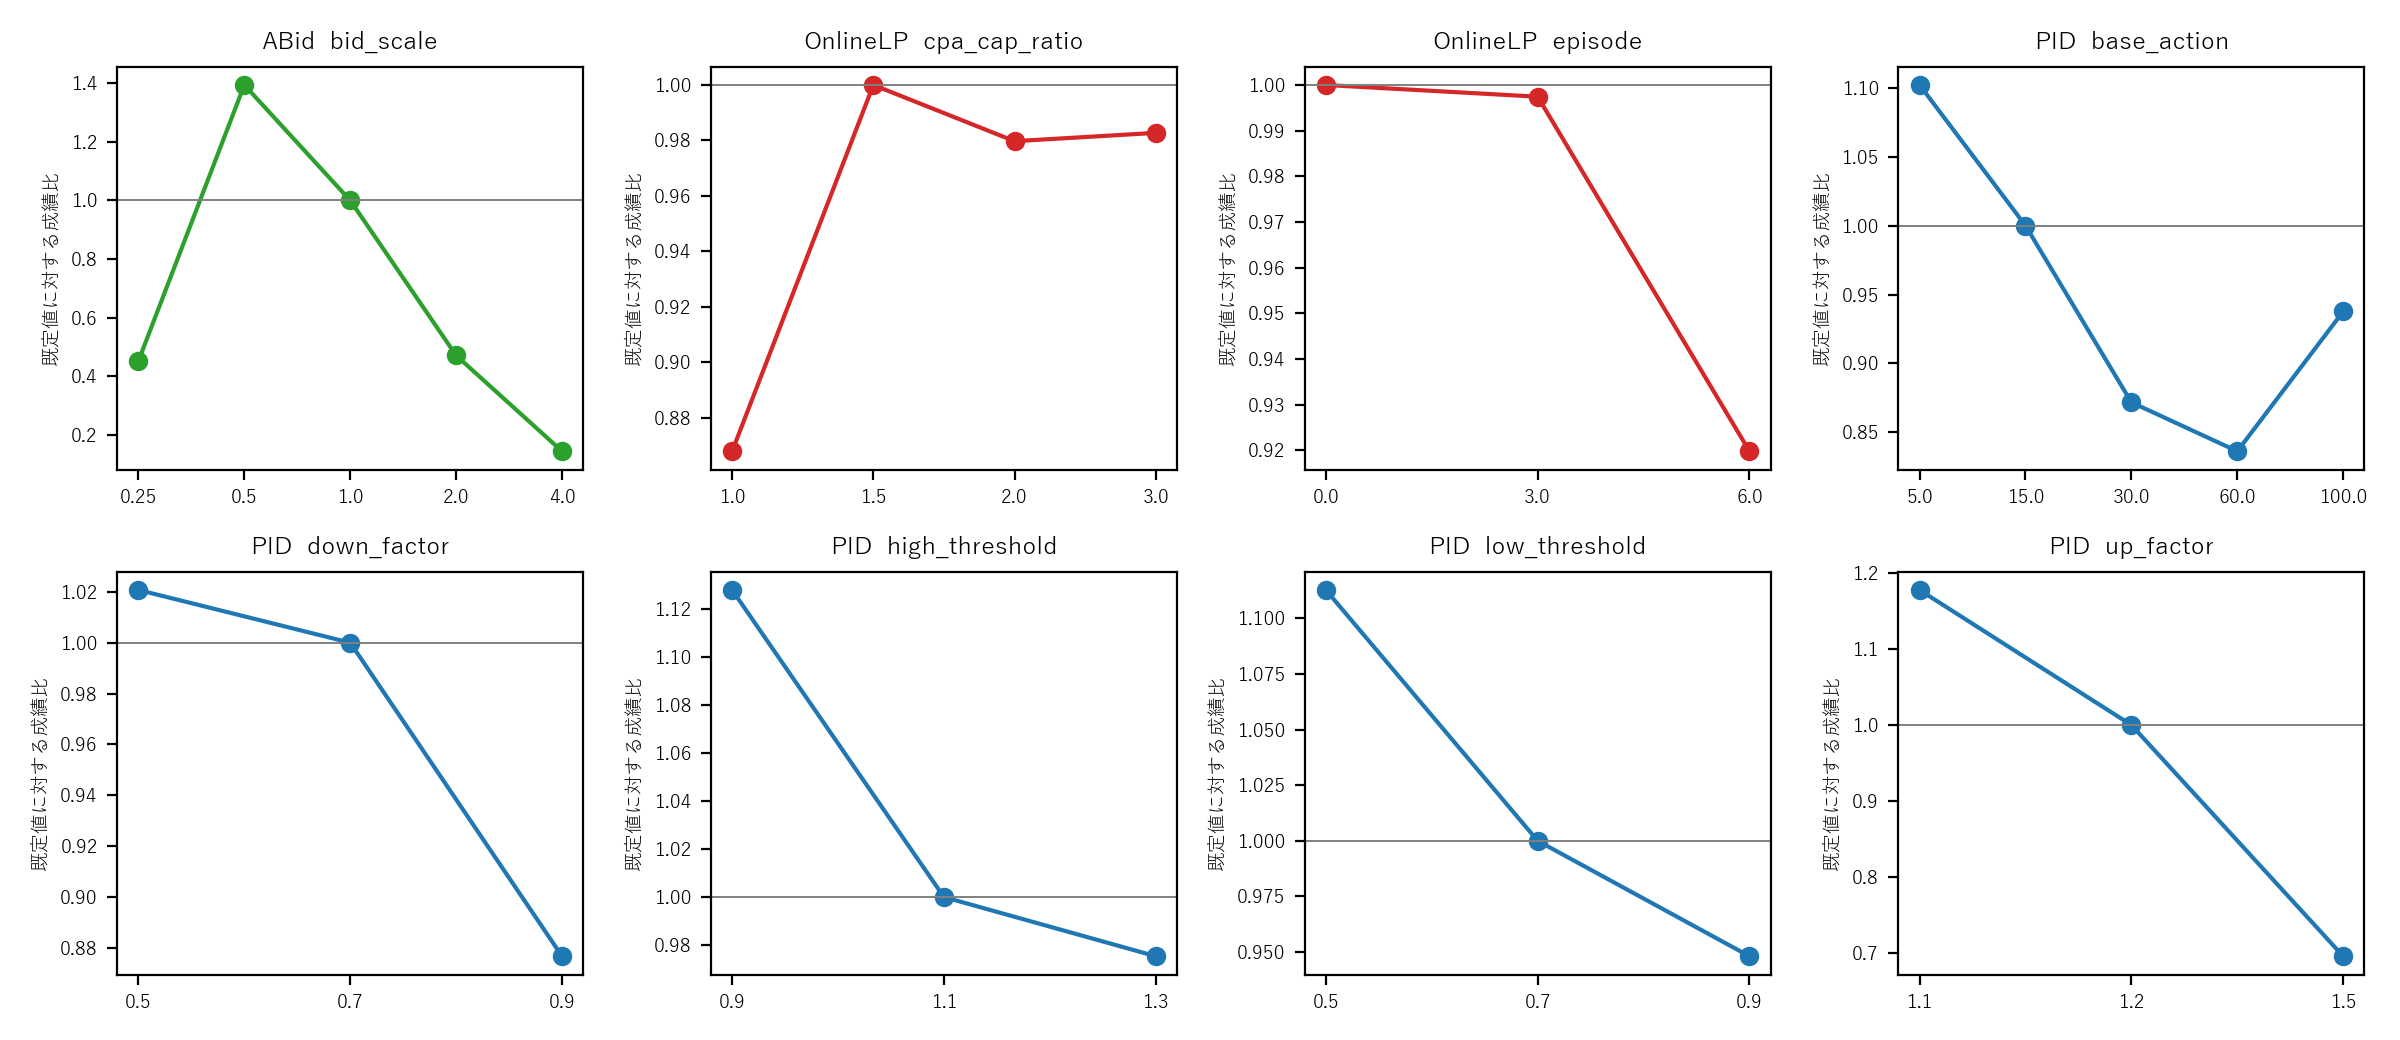
\includegraphics[width=0.8\textwidth]{fig/fig_sweeps.png}
\caption{パラメータ掃引（6位置×4エピソードの平均scoreの，既定値に対する比。横軸は振った値）}
\label{fig:sweeps}
\end{figure*}

\subsection{実験環境}\label{sec:e-env}

48社のうち1社（プレイヤー）を対象の手法に差し替え，残りの47社は環境に同梱の手法のままにした（表\ref{tab:cond}）。
成績は，エピソードごとの「購入数$\times$ペナルティ係数」（以下，score）で見る。
ペナルティ係数は，実績CPAが制約を超えたときだけ（制約$\div$実績CPA）$^2$になり，超えなければ1である。

\begin{table}[H]
\centering
\caption{実験の条件（1 run$=$1位置$\times$4エピソード）}
\label{tab:cond}
\footnotesize
\begin{tabularx}{\linewidth}{@{}l>{\raggedright\arraybackslash}X@{}}
\toprule
固定 & シミュレータは既定の設定，乱数seed=1 \\
 & Windows 11，Python 3.9.25，CPU \\
\midrule
比較 & 3手法（既定のパラメータ） \\
 & 位置48$\times$エピソード0〜3（192セル） \\
 & 計144 run \\
\midrule
掃引 & パラメータを1つずつ振る（他は既定） \\
 & 位置0, 8, 16, 24, 32, 40$\times$エピソード0〜3 \\
 & PID：最初の$\alpha$，上げ下げの倍率，2つの閾値 \\
 & ABid：全体の倍率 \\
 & Online LP：$\alpha$の上限，早見表の日 \\
 & 計126 run \\
\bottomrule
\end{tabularx}
\end{table}

\subsection{取った特徴量}\label{sec:e-feat}

成績のほかに，あとから原因を考えるための量を，ティックごとに記録した（表\ref{tab:feat}）。

\begin{table}[H]
\centering
\caption{取った特徴量}
\label{tab:feat}
\footnotesize
\begin{tabularx}{\linewidth}{@{}l>{\raggedright\arraybackslash}X@{}}
\toprule
種類 & 記録した量 \\
\midrule
入札の強さ & 実効の$\alpha$（入札額の和$\div$価値の和），その順位，他47社の$\alpha$の中央値 \\
市場 & 最低落札価格，予算が残る広告主の数，全体の支出 \\
予算のペース & 支払い，残り予算，PV数，予算消化率，最後に落札したティック \\
落札の中身 & 落札数（スロット別），露出数，価値の平均とばらつき \\
CPA & 実績CPA，ペナルティ係数，ペナルティ前の購入数 \\
位置と他社 & 予算，CPA制約，カテゴリ，全48社の成績と順位 \\
規模 & 所要時間（全体，\texttt{bidding()}1回），最大メモリ \\
\bottomrule
\end{tabularx}
\end{table}

% ============================================================
\section{結果}\label{sec:e-result}
% ============================================================

\textbf{動作}　270 run（PID 120，ABid 72，Online LP 78）が，すべて完走し，scoreは有限であった。
1回目に掃引の13 runがメモリ不足で失敗した（8並列に加えて集計を同時に走らせた）。6並列で流し直すと，13 runとも完走した。

\textbf{規模感}　1 run（1位置×4エピソード）は，6〜8並列でPID 210秒，ABid 215秒，Online LP 204秒（1エピソード約51〜54秒）で，
4並列のときは約150秒であった。最大メモリは1プロセス約2.5GBであった。
\texttt{bidding()}1回の平均は，PID 0.12ms，ABid 0.25ms，Online LP 1.66ms，1回の最大は1.9ms，2.3ms，9.4msであった（図\ref{fig:scale}）。

\begin{figure}[H]
\centering
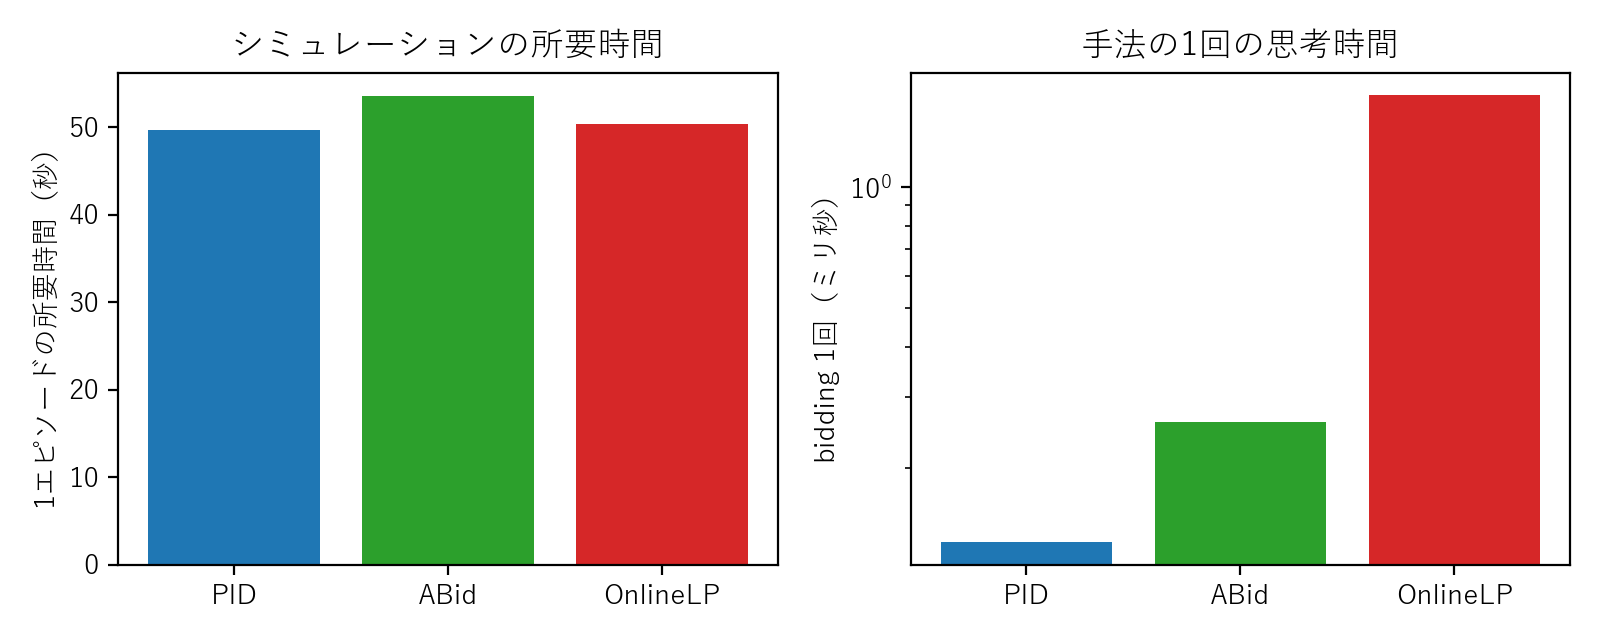
\includegraphics[width=0.9\linewidth]{fig/fig_scale.png}
\caption{所要時間。左：1エピソードのシミュレーション，右：\texttt{bidding()}1回（対数軸）}
\label{fig:scale}
\end{figure}

\textbf{再現性}　同じ設定の再実行で，\texttt{episodes}表の全列が全エピソードで完全に一致した（報酬・scoreの差は0.0）。

\textbf{3手法の比較}　表\ref{tab:cmp}と図\ref{fig:scores}のとおり，Online LPのscore合計は，PIDの1.92倍，ABidの1.49倍で最大であった（論文の「Online LPが最良」と同じ向き）。
なお，論文の図10（目視の概算）ではPIDはAbidの2〜3.5倍，Online LPは6〜7倍であり，本結果（PID 0.78倍，Online LP 1.49倍）とは，PIDとAbidの順序と倍率が一致しない（原因は未確認）。
セル単位でOnline LPがPIDを上回った割合は0.77，ABidを上回った割合は0.69，PIDがABidを上回った割合は0.42であった。
6カテゴリごと，4エピソードごとの合計は，すべてOnline LPが最大であった。
プレイヤー以外の47社の平均スコアは，手法によらず21.3〜21.4でほぼ同じであった。

\begin{table}[H]
\centering
\caption{既定設定の3手法（48位置×4エピソード，192セル）}
\label{tab:cmp}
\footnotesize
\begin{tabularx}{\linewidth}{@{}Xrrr@{}}
\toprule
 & ABid & PID & Online LP \\
\midrule
score合計（÷20000） & 0.165 & 0.128 & 0.246 \\
ABidを1.0とした値 & 1.00 & 0.78 & 1.49 \\
平均報酬（ペナルティ前） & 25.8 & 24.4 & 28.7 \\
ペナルティが掛かったセルの割合 & 0.85 & 0.82 & 0.39 \\
予算消化率の平均 & 0.93 & 0.99 & 0.75 \\
最終ティックより前に落札が止まった割合 & 0.81 & 0.56 & 0.41 \\
順位の中央値 & 32 & 35 & 18 \\
\bottomrule
\end{tabularx}
\end{table}

\begin{figure}[H]
\centering
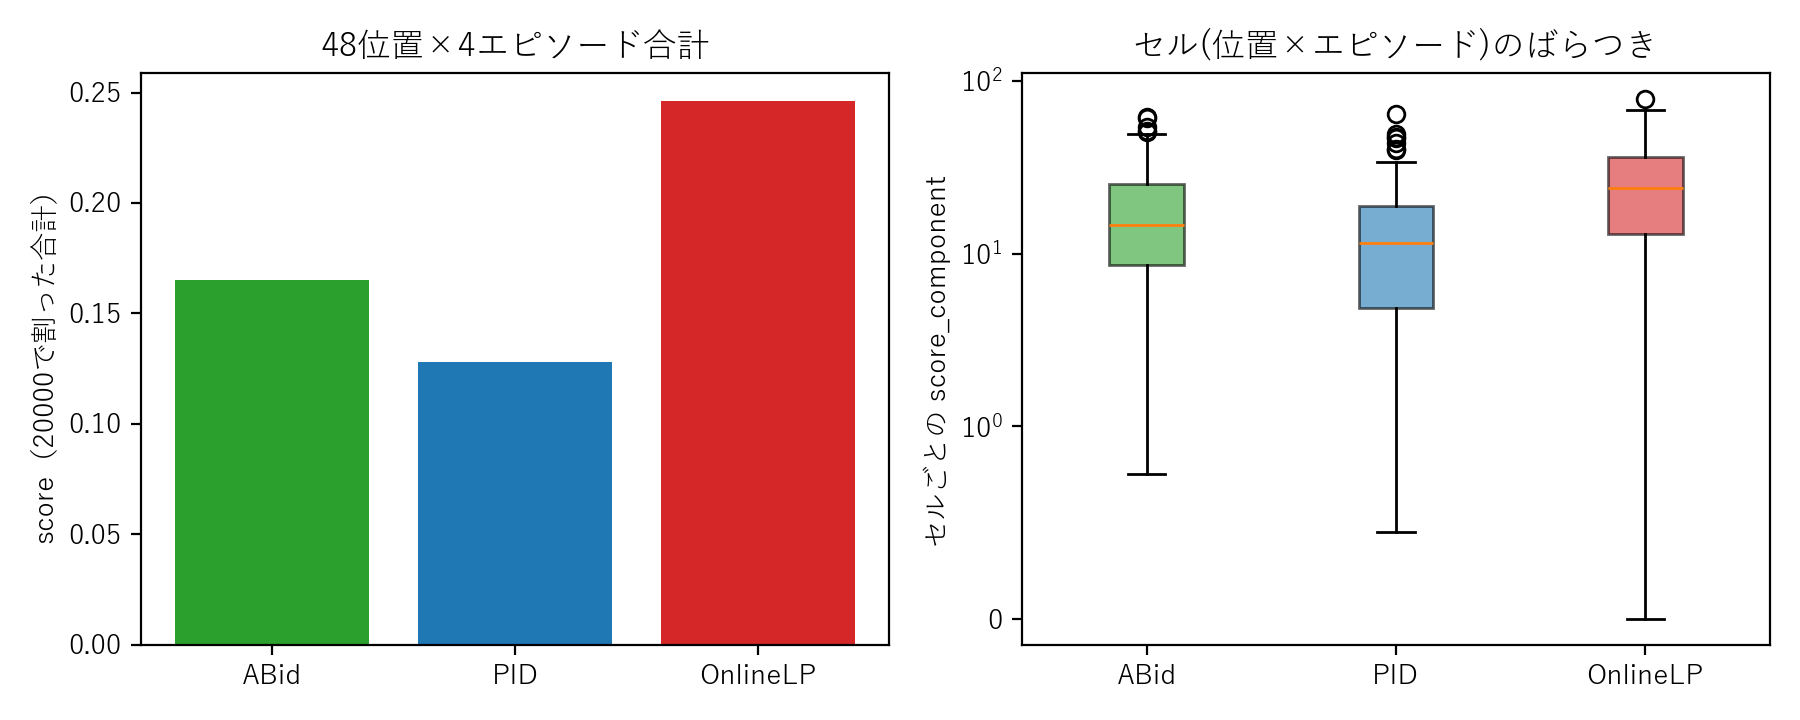
\includegraphics[width=\linewidth]{fig/fig_scores.png}
\caption{3手法のスコア。左：合計，右：セルごとの分布（symlog軸）}
\label{fig:scores}
\end{figure}

図\ref{fig:alpha}は，実効入札係数$\alpha$（入札額の和÷価値の和）などの時系列である。
PIDはティック0の$\alpha$が15で（他47社の中央値は68），落札数が0から立ち上がるのはティック7ごろ以降であった。
ABidはティック0〜20の$\alpha$が約115で，ティック23以降の中央値は0であった。
Online LPは全ティックで70〜89に収まり，他47社の中央値に近かった。


\textbf{パラメータ掃引}　図\ref{fig:sweeps}のとおり，振った範囲で最良点が既定値だったのは，Online LPの2つのパラメータだけであった。
既定値に対する最良点の比は，PIDで1.02〜1.18（\texttt{up\_factor}を1.2から1.1にすると1.18），ABidで1.39（\texttt{bid\_scale}を1から0.5にすると），
Online LPで1.00であった。ABidは入札倍率を0.25にすると0.45倍，4にすると0.14倍に落ちた。
同じ6位置で，既定のOnline LPは23.4，PIDの最良点は18.2，ABidの最良点は17.0であった。


\textbf{特徴量}　\texttt{episodes}（1,028行），\texttt{ticks}（49,344行），\texttt{agents}（49,344行）の全数値列に，NaN・無限大はなかった。

以上より，実験の前に決めた達成条件（REP001.md）をすべて満たし，探索の目的は\textbf{達成}した。

\end{document}
